\chapter{Simulations}
\label{ch:simulations}

\section{Introduction}

In order to test algorithm ideas, one would either have to implement them as a prototype and run it on significant number of nodes, hoping that the results would scale in predictable way in relation to how node count changes. The other way is to create a simulator, which given input parameters - for example, the number of nodes, number of jobs and quality of nodes - would be able to estimate performance of the grid over time.

Simulator created for this thesis is able to test how would hypothetical computing grid behave, if jobs scheduling and trust management were implemented with presented methods and algorithms. The simulators are able to simulate dynamics of grid network during computation of one project. Network data, such as nodes' trust, times of completion and number of confirmations of jobs is collected.

Both simulators are implemented in C++, depending on standard C++ library. Parallel simulator uses OpenMPI. Gnuplot is used, along with gnuplot-iostream~\cite{gp-iostream} to plot the resulting data.

\section{Simulator design}

Simulator understands the notion of \emph{Nodes}, \emph{Jobs}, and \emph{Results}. Additionally, \emph{AssumedResult} is defined as the result that is hoped to be delivered by Node, but is not ready yet.

Node is described by:
\begin{itemize}
\item Performance - how quickly the node is able to generate new results.
\item Trust - current accumulated amount of trust from the confirming results.
\item Current job - job the node is currently computing.
\item Submitted results - collection of all submitted results.
\end{itemize}

Job is defined as:
\begin{itemize}
\item Difficulty - how difficult the task is to compute, that is, how much prelonged computation will be.
\item Results - collection of results already delivered.
\item Assumed results - collection of results that are hoped to be delivered.
\end{itemize}

Result is defined by \emph{hash}, which tells what kind of result it is. Hash value of 0 is considered as a correct result. Any other value makes the result to be considered incorrect, but the results with same hash value confirm one another. So enough incorrect but same results will be accepted as correct by the network, potentially disturbing its progress.

Each result is related to exactly one Node and exactly one Job. Result's \emph{correctness} is defined to be \emph{trust} of the \emph{node} at the time of submitting the result.

Relations between described classes are also shown on figure~\ref{f:simclassdg}.

\begin{figure}
\centering
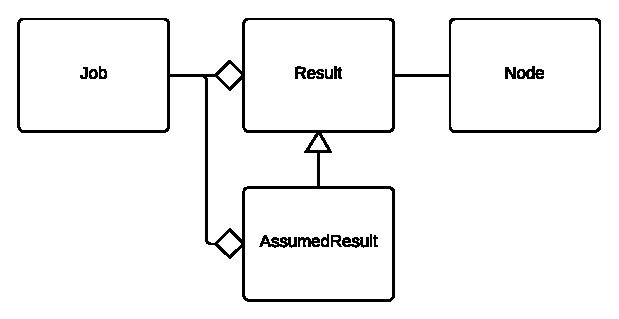
\includegraphics{diagrams/SimulatorClassDiagram.pdf}
\caption{Diagram of classes used in the simulator.}
\label{f:simclassdg}
\end{figure}

\section{Simulator loop}

Simulation is done by evaluating each node in a loop. Time is represented by abstract time unit. Every iteration of the loop is simulation of network in consecutive time units - \emph{tick}. In each iteration of loop, every node is evaluated, by doing as follows:
\begin{itemize}
	\item If node is working on idling, continue to the next node.
	\item If not: \begin{itemize}
		\item If node has just finished job, hand out job, recompute job's correctness and participants' trust.
		\item Find a new job for the node. \begin{itemize}
			\item If job is found, calculate work time.
			\item If no job is found, set to idle until next tick. 
		\end{itemize}
	\end{itemize}
\end{itemize}

The ticks are being simulated until all jobs are estimated to be complete. Job is complete when a set of results can be found which have the same \emph{hash} and sum of their \emph{correctness} exceeds $1$.

Upon each iteration, we can plot data such as nodes' trust or percent of completed jobs. Simulator uses gnuplot for this task.

\section{Implementation}

In order to achieve highest performance possible, appropriate data structures are used. This section will explain how certain performance critical aspects of simulator are implemented and the rationale behind it.

Set is used as a data structure to keep collection of objects. Ordered set can keep unique elements following a specific order. Operations on sets, such as searching for elements and inserting an element, are of logarithmic complexity.

\subsection{Nodes}

The node collection is an ordered set, where the order is determined by \emph{next working tick}. \emph{Next working tick} is the tick when the node state should change. When a node gets job at tick $10$ and the job is calculated to take $5$ ticks, \emph{next working tick} is $15$. At tick $15$ job will be finished, nodes' trust recalculated and node will get new job. There is no need to check on node during ticks $11$ to $14$.

\begin{figure}
\centering
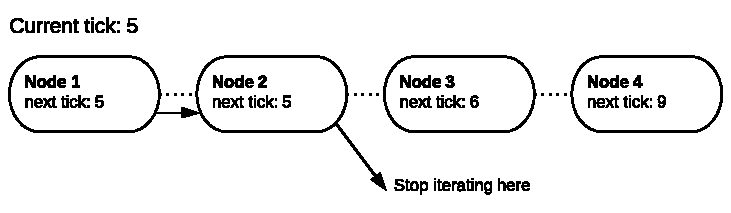
\includegraphics{diagrams/SimulatorNodes.pdf}
\caption{Iterating through simulator nodes. Simulator breaks out of the loop early, skipping nodes that should not be processed in current iteration.}
\label{f:simnodes}
\end{figure}

Because iteration happens on ordered set of nodes, we can stop iterating as soon as we reach node that \emph{next working tick} is higher than current tick. Example of this behavior is shown in figure~\ref{f:simnodes}. The only thing to keep in mind is to reinsert node (to update its position in set and keep data structure consistency) when node state is changed and therefore \emph{next working tick} changes.

\subsection{Jobs}

Jobs are kept in ordered set with the order determined by jobs current best correctness, but in reverse. Jobs with highest correctness are first. Because we search a job for nodes very often, it can become performance bottleneck. 

Jobs are selected in a way that node's contribution will get job closer to completion, which is determined by sum of trust of confirmed results of $1$, but also trying not to waste node's computing power. Waste is considered when sum of correctness exceeds $1$ by significant amount. For example, when job's best correctness is $0.8$, there is no reason to give this job again for a node with trust of $0.5$. Node with $0.2$ trust will suffice.

Ordered set of jobs allows us to use bisection to find best matching job. It may happen that the job cannot be given to this particular node, because it already has sent result for it. If so, we start iterating from that node until we find one that we can give to the node.